\documentclass[12pt]{article}

\usepackage[style=phys,citestyle=authoryear,maxcitenames=2]{biblatex}
\addbibresource{stats-report.bib}

\usepackage[page]{appendix}

\usepackage{amsmath,amssymb,commath,mathabx,mathtools,physics,siunitx}
\usepackage{aas_macros}
\usepackage{float,subcaption}

\usepackage[margin=1in]{geometry}
\usepackage{setspace}
\doublespacing

\title{
  Working Title
}

\author{
  Jacob Lange, Chi Nguyen, Daniel Wysocki
}

\date{
  Statistical Methods for Astrophysical Sciences (ASTP-611)
  \\
  Spring 2016
}



\begin{document}

\maketitle


\begin{abstract}


\end{abstract}


\section{Introduction}
\label{sec:intro}
The detection of gravitational waves (GW) in Feburary(ref) opened a new era of astronomy; however, it is only in sync with electromagnetic astronomy that the most physics can be discovered. Electromagnetic counterparts are expected from binary sources involving matter i.e. neutron star-neutron star and neutron star-black hole. Because of this, GW detectors will work in conjunction with electromagnetic telescopes to observe a GW source. Some of these will yield weak, nearly isotropic electromagnetic counterparts and others will not. GW detectors will identify sources characterized by its chirp mass:

\begin{equation}
M_{c}=\frac{(m_{1}m_{2})^{3/5}}{(m_{1}+m_{2})}
\end{equation}

Figure \ref{fig:chirp} is the full data set in terms of chirp mass. The electromagnetic counterparts events are seperated from the other events by color. This report is organized as follows. Section \ref{sec:dist} describes the developement of the chirp mass distribution, Section \ref{sec:classifier} descibes a electromagnetic followup classifier based on the data, and Section 4 will state our conclusions.
\begin{figure}
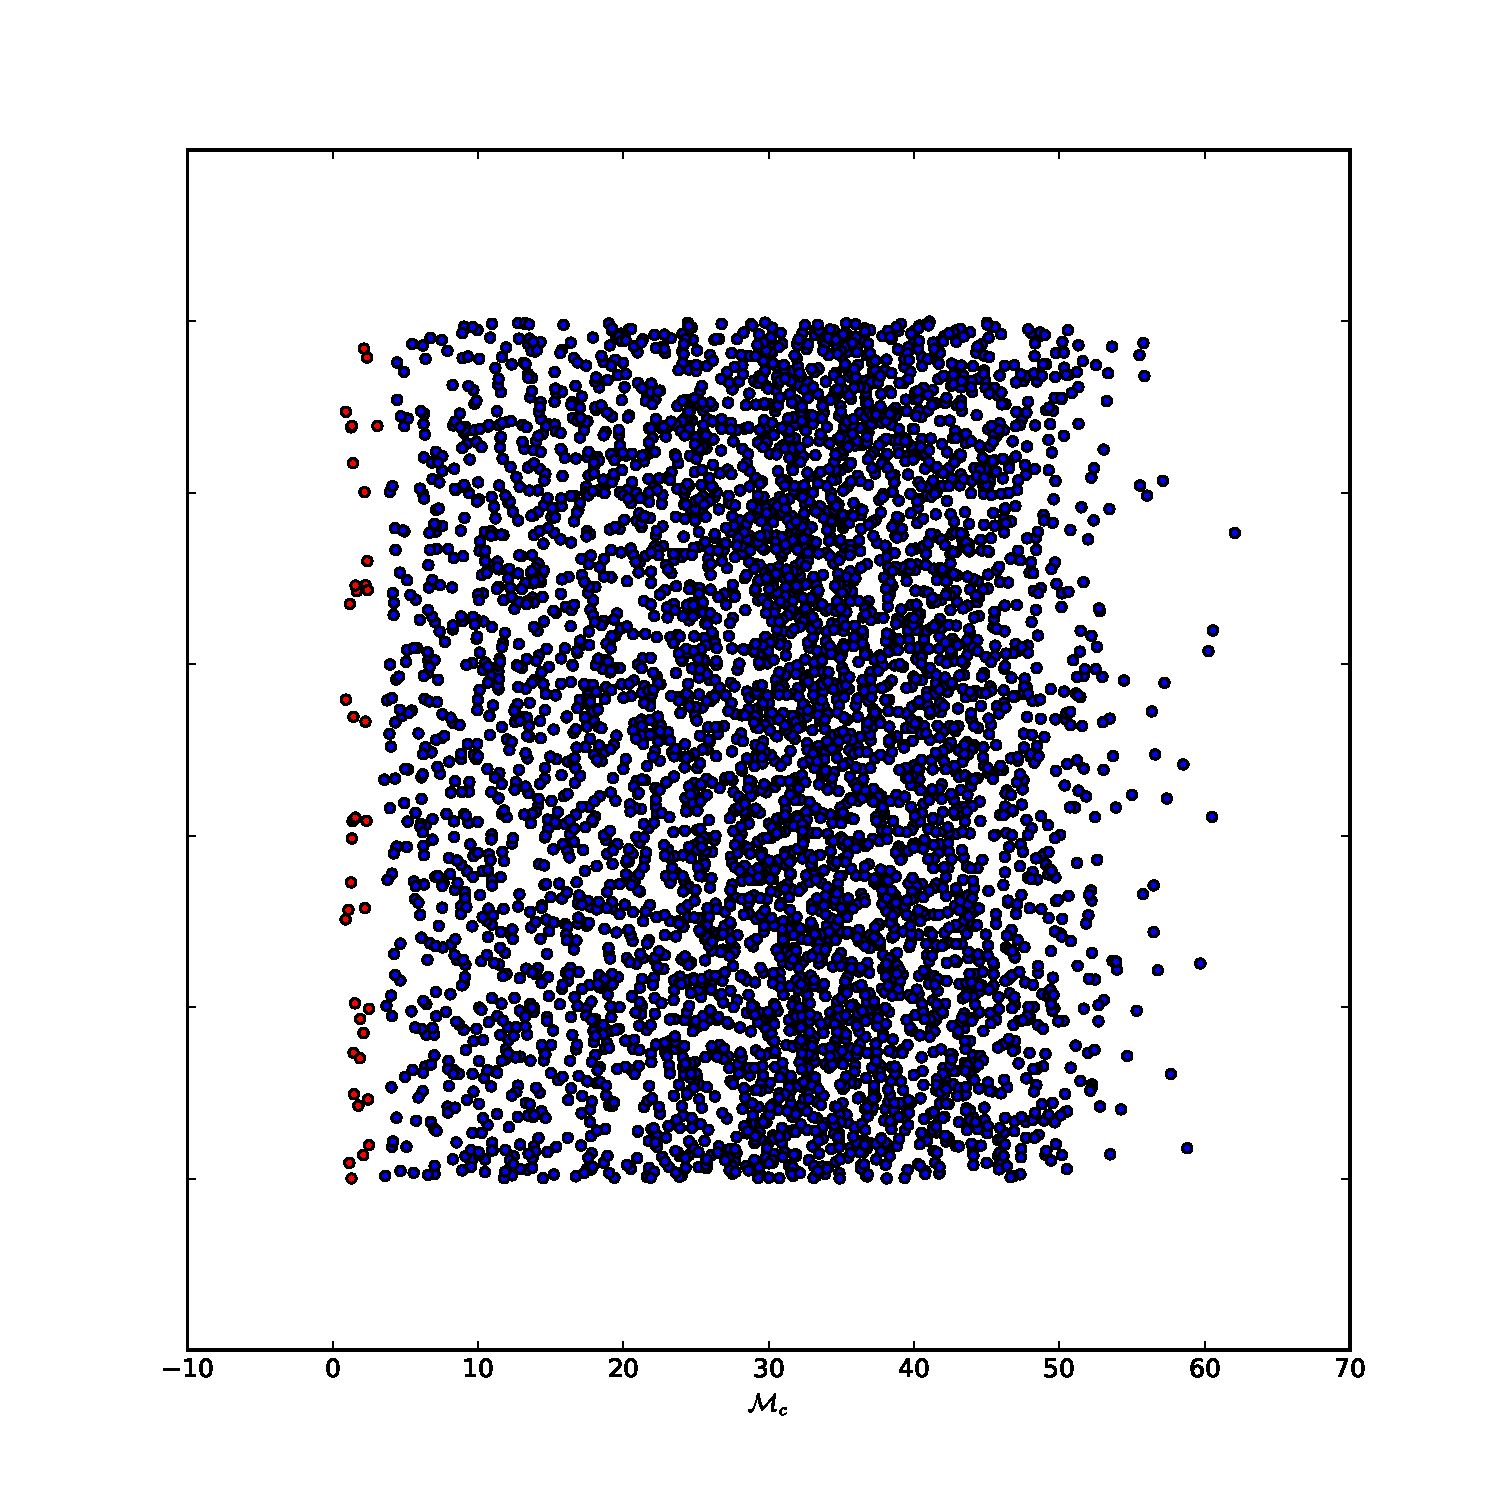
\includegraphics[width=\columnwidth]{output/jake/chirp-mass-classes.pdf}
\caption{This figure shows all the 5000 events' chirp mass. Here the y-axis is a uniform random number between zero and one. The events that have an electromagnetic counterpart are in red, and the events without a electromagnetic counterpart are in blue.}
\label{fig:chirp}
\end{figure}
See Section \ref{sec:discussion} and Appendix \ref{app:example}. Example text citation is \textcite{2012ApJ...759...52D}, or in parenthesis with a page number \parencite[pg 2]{2012ApJ...759...52D}.


\section{Chirp Mass Distribution}
\label{sec:dist}





\section{Classifying GW Events that have Electromagnetic Countparts}
\label{sec:classifier}
The GW observatory, the Laser Interferometer Gravitational Wave Observatory (LIGO), can provide very rapid mass estimates of candidate GW events. Since most of these detections are mostly binary black holes and electromagnetic followup is extremely expensive, only a few events can be followed up. We have therefore trained a classifier to determine if an event will have a electromagnetic followup. We trained this classifier on the first half of the data. We simply took the mid-way point betweewn the maximum chirp mass for the electromagnetic counterpart group and the other group. This is shown in Figure \ref{fig:half}. This was then used on the whole dataset as shown in Figure \ref{fig:all}.

\begin{figure}
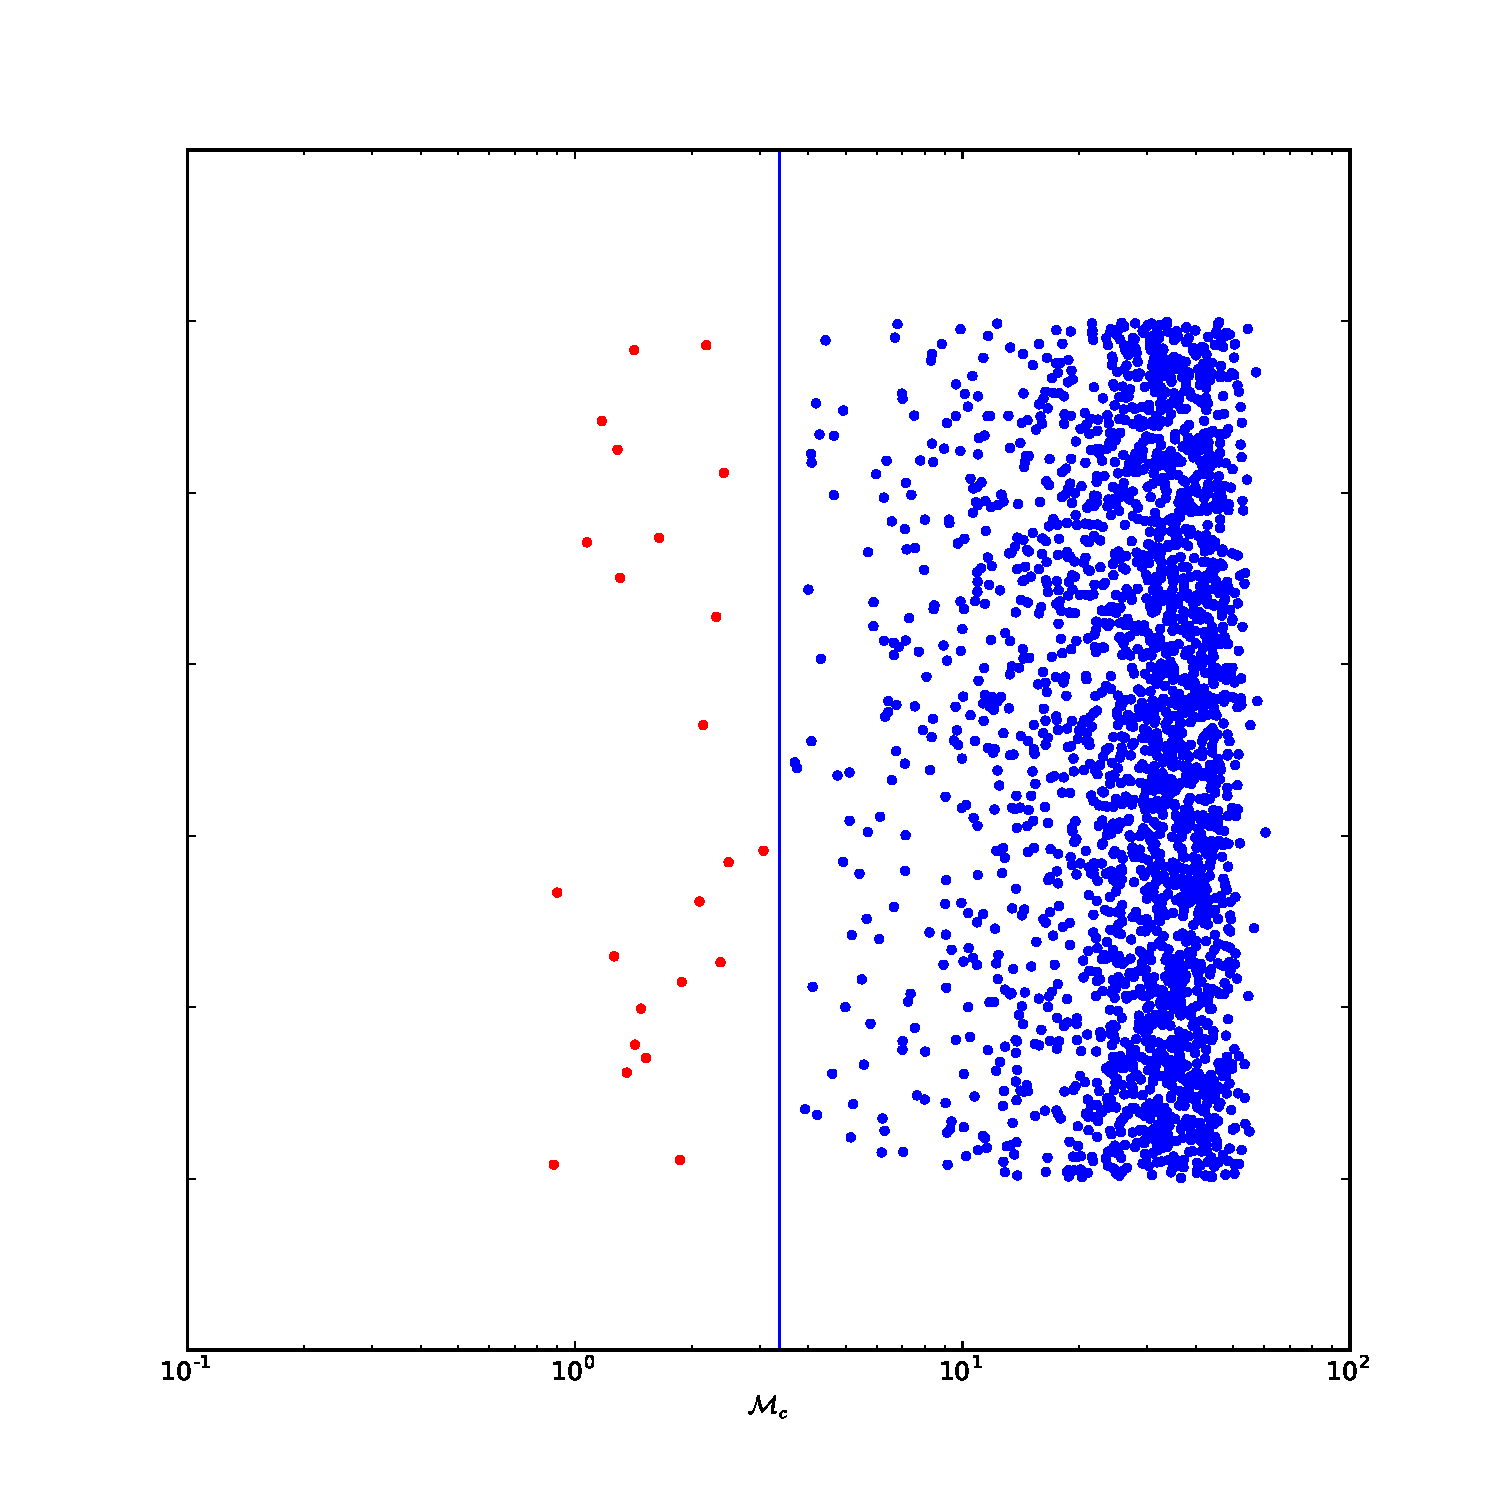
\includegraphics[width=\columnwidth]{output/jake/classifier_half.pdf}
\caption{This shows the first half of the data with the same two groups as before. The vertical line indicates the division between the two groups.}
\label{fig:half}
\end{figure}
\begin{figure}
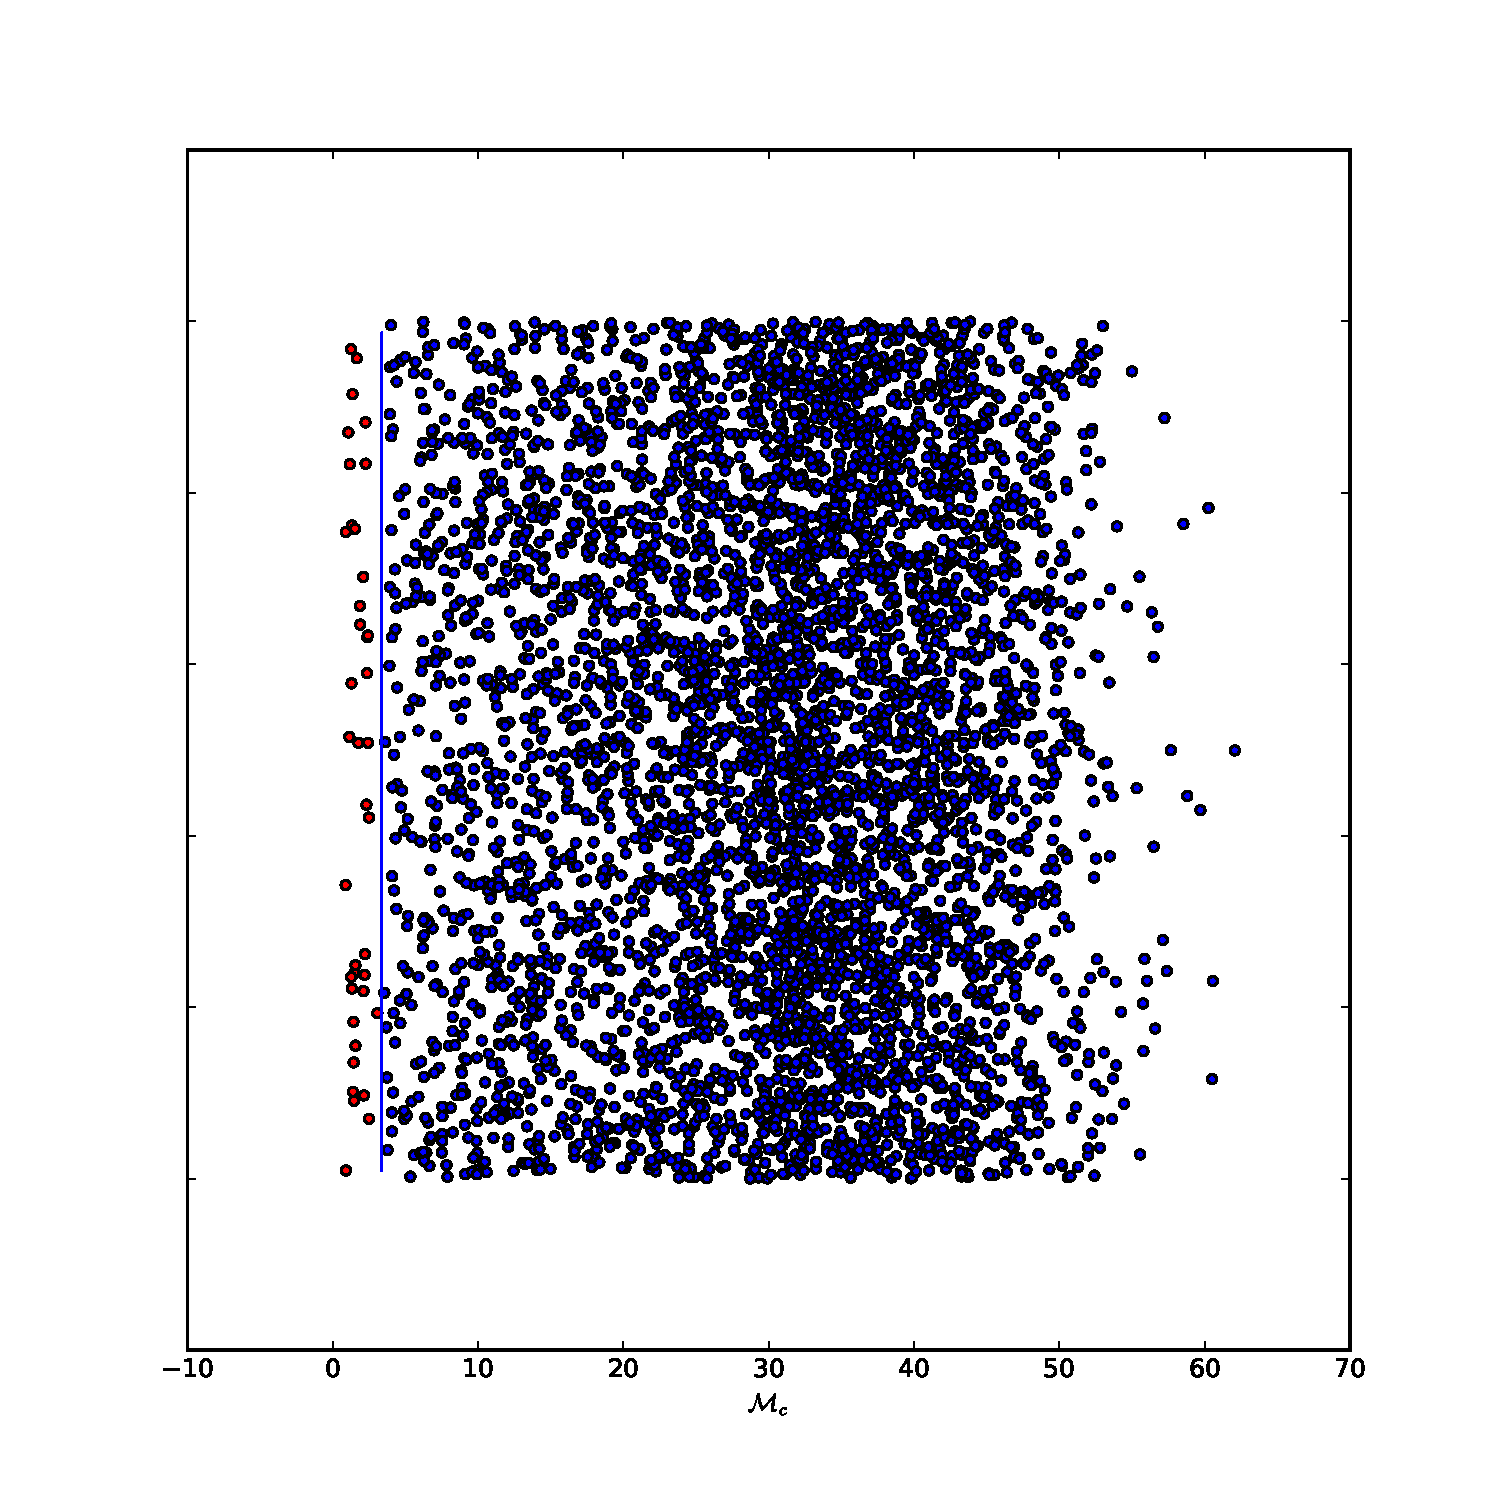
\includegraphics[width=\columnwidth]{output/jake/classifier_all.pdf}
\caption{This shows the full set of the data with the dividing line trained by half the data.}
\label{fig:all}
\end{figure}



\section{Conclusions}
\label{sec:conclusions}




\printbibliography[heading=subbibliography]

\begin{appendices}

\section{Example}
\label{app:example}


\end{appendices}






\end{document}